\section{Single spin}
\subsection{Precession of spin in uniform magnetic field}

We simulate the time evolution of a single spin $\mathbf{S}$ in the presence of a uniform magnetic field $\mathbf{B} = (0,0,B_0)^T$ in the $\mathbf{e}_z$-direction. The components of the spin at equidistant time steps during one period are shown in figure \ref{fig:spin_1}. As expected, we see that the spin precesses around the effective field $\mathbf{H}$, which in this case is given by
\[
	\mathbf{H} = -\pd{H}{\mathbf{S}} = \frac{\partial}{\partial \mathbf{S}}\left( \mu \mathbf{B} \cdot \mathbf{S} \right) =\mu \mathbf{B},
\]
in the absence of damping and anisotropy.

\begin{figure}[htb]
	\centering
	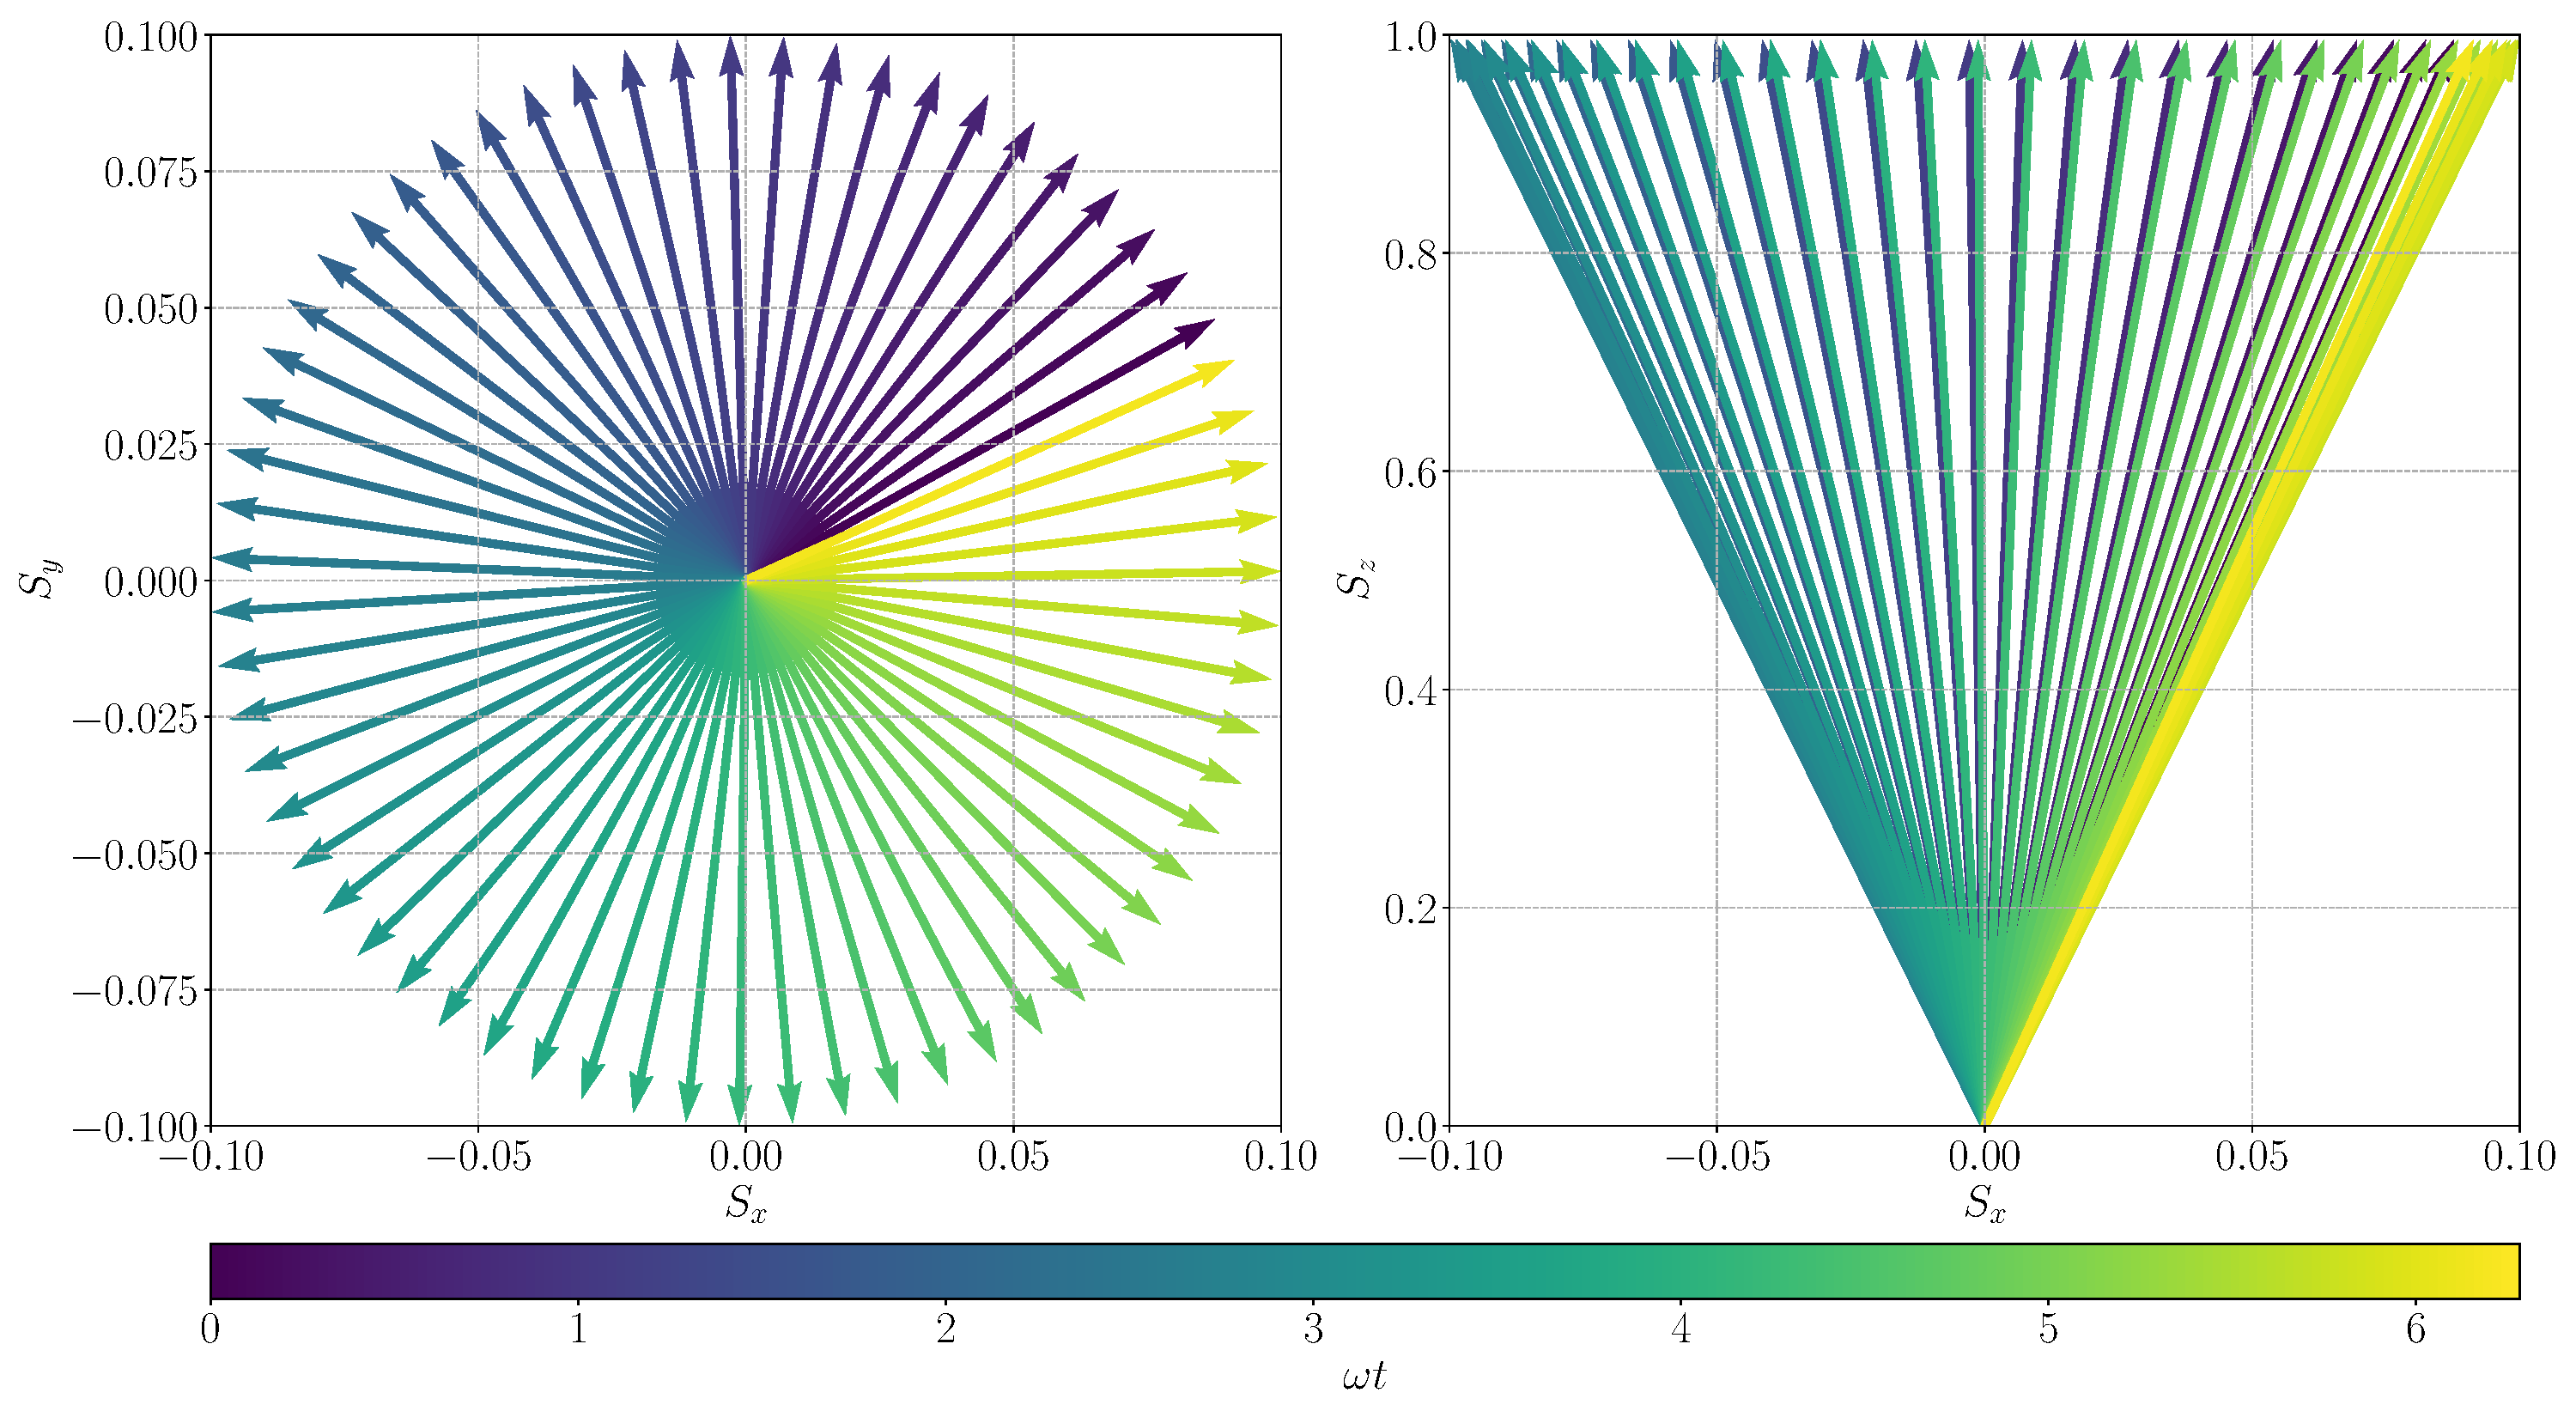
\includegraphics[width=\columnwidth]{../fig/magnet_xy_1}
	\caption{The figure shows the $x$ and $y$ component of the spin during one period in a uniform magnetic field without further interactions.}
	\label{fig:spin_1}
\end{figure}

In this particular case, we can easily find an analytical solution to compare with. The LLG-equation reads
\[
	\partial_t \mathbf{S} = -\frac{\gamma}{\mu} \mathbf{S} \times \mathbf{B}.
\]
As $\mathbf{B} = (0,0,B_0)^T$,
\[
	\mathbf{S} \times \mathbf{B} = (S_y \mathbf{e}_x - S_x \mathbf{e}_y) B_0.
\]
Thus, we have two equations 
\begin{equation}\label{eq:eq_sys}
	\begin{cases}
		\partial_t S_x = -\gamma B_0 S_y \\
		\partial_t S_y = \gamma B_0S_x.
	\end{cases}
\end{equation}
which are easily solved by differentiating both with respect to $t$, and then substituting the first order derivatives on the right hand side by the corresponding expressions in \ref{eq:eq_sys}.
\begin{equation}
	\begin{cases}
		\partial^2_t S_x = -\gamma B_0 \partial_t S_y  \\
		\partial^2_t S_y = \gamma B_0 \partial_t S_x.
	\end{cases}
\end{equation}
This yields the two equations
\begin{equation}
	\ddot{S}_x = - \left( \gamma B_0 \right)^2 S_x \quad;\quad \ddot{S}_y = - \left( \gamma B_0 \right)^2 S_y, 
\end{equation}
which have solutions 
\begin{align}
	S_x(t) &= S_x(0) \cos{(\omega t)} - S_y(0) \sin{(\omega t)} \label{eq:exact_1} \\
	S_y(t) &= S_y(0) \cos{(\omega t)} + S_x(0) \sin{(\omega t)} \label{eq:exact_2},
\end{align}

with the frequency $\omega = \gamma B_0$. When comparing the exact solution with the numerical estimate obtained through integrating the LLG-equation with Heun's method, the trajectories of $S_x$ and $S_y$ are as shown in figure \ref{fig:comp}.

\begin{figure}[htb]
	\centering
	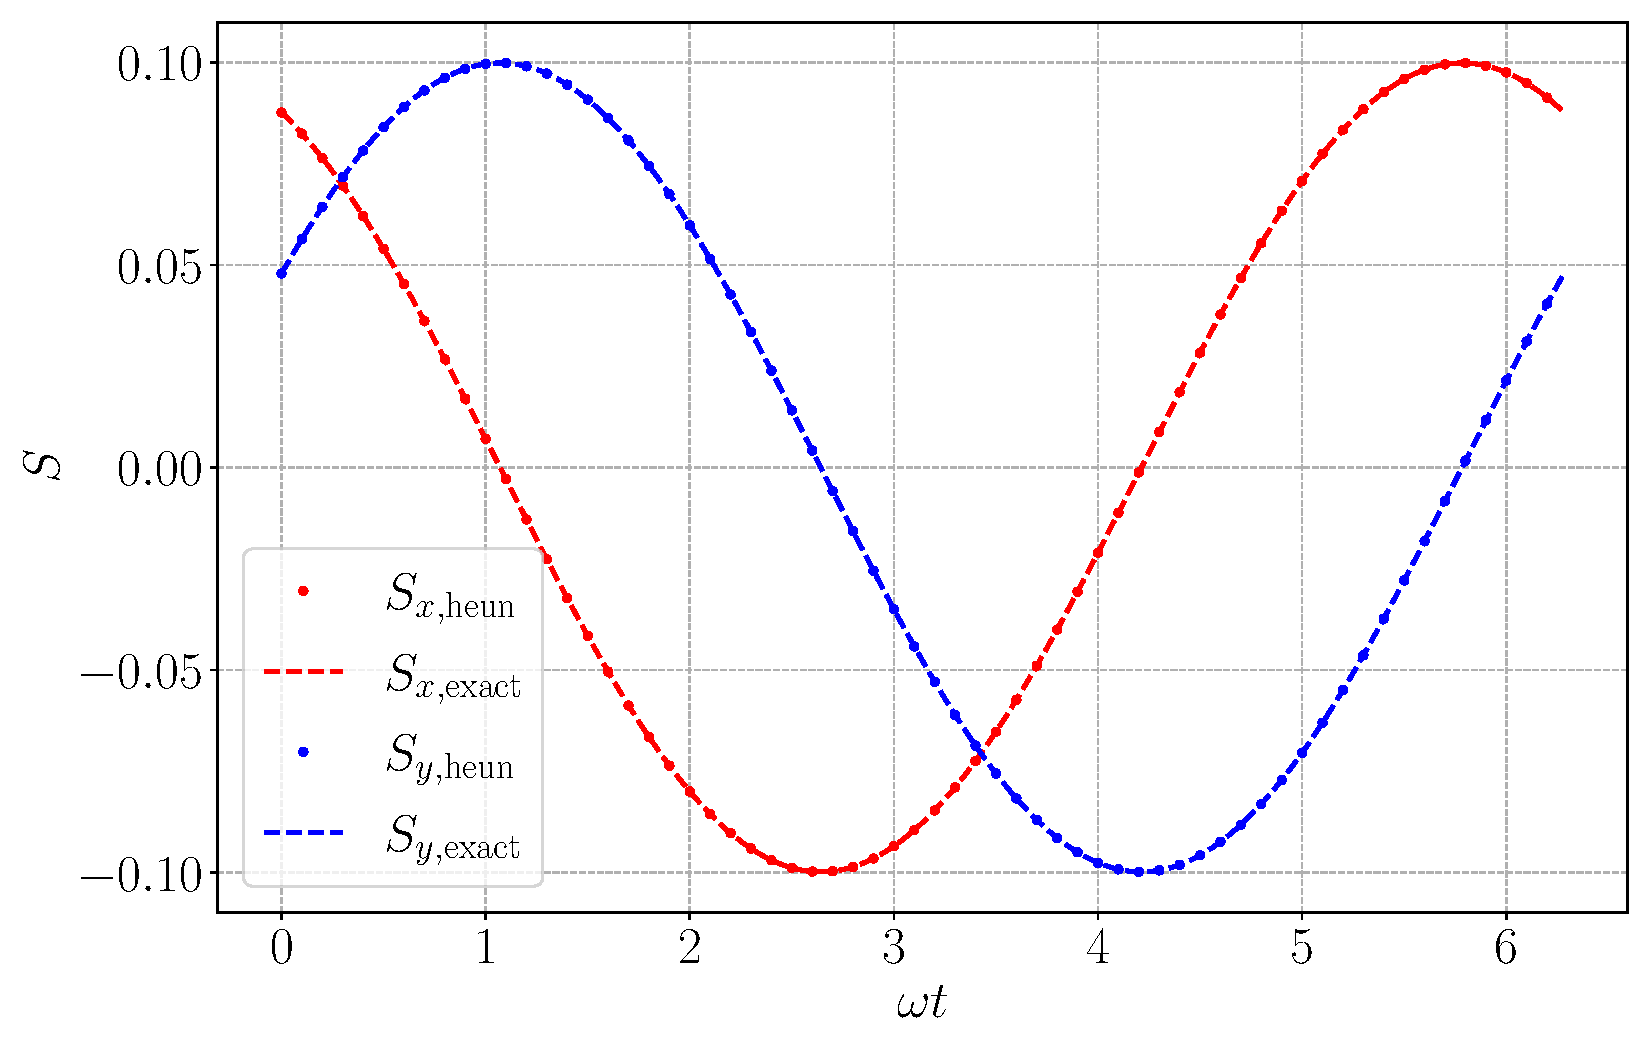
\includegraphics[width=\columnwidth]{../fig/comparison.pdf}
	\caption{The plot shows the exact solution given in \eqref{eq:exact_1} and \eqref{eq:exact_2} compared with the numerical solution sampled at every tenth step to be able to distinguish the paths.}
	\label{fig:comp}
\end{figure} 

It is perhaps more enlightening to consider the pointwise difference of the exact and numerical solution. This is shown in figure \ref{fig:comp_diff}. The figure shows that the deviations locally oscillate, but globally, of course, the absolute deviation increases.

\begin{figure}[htb]
	\centering
	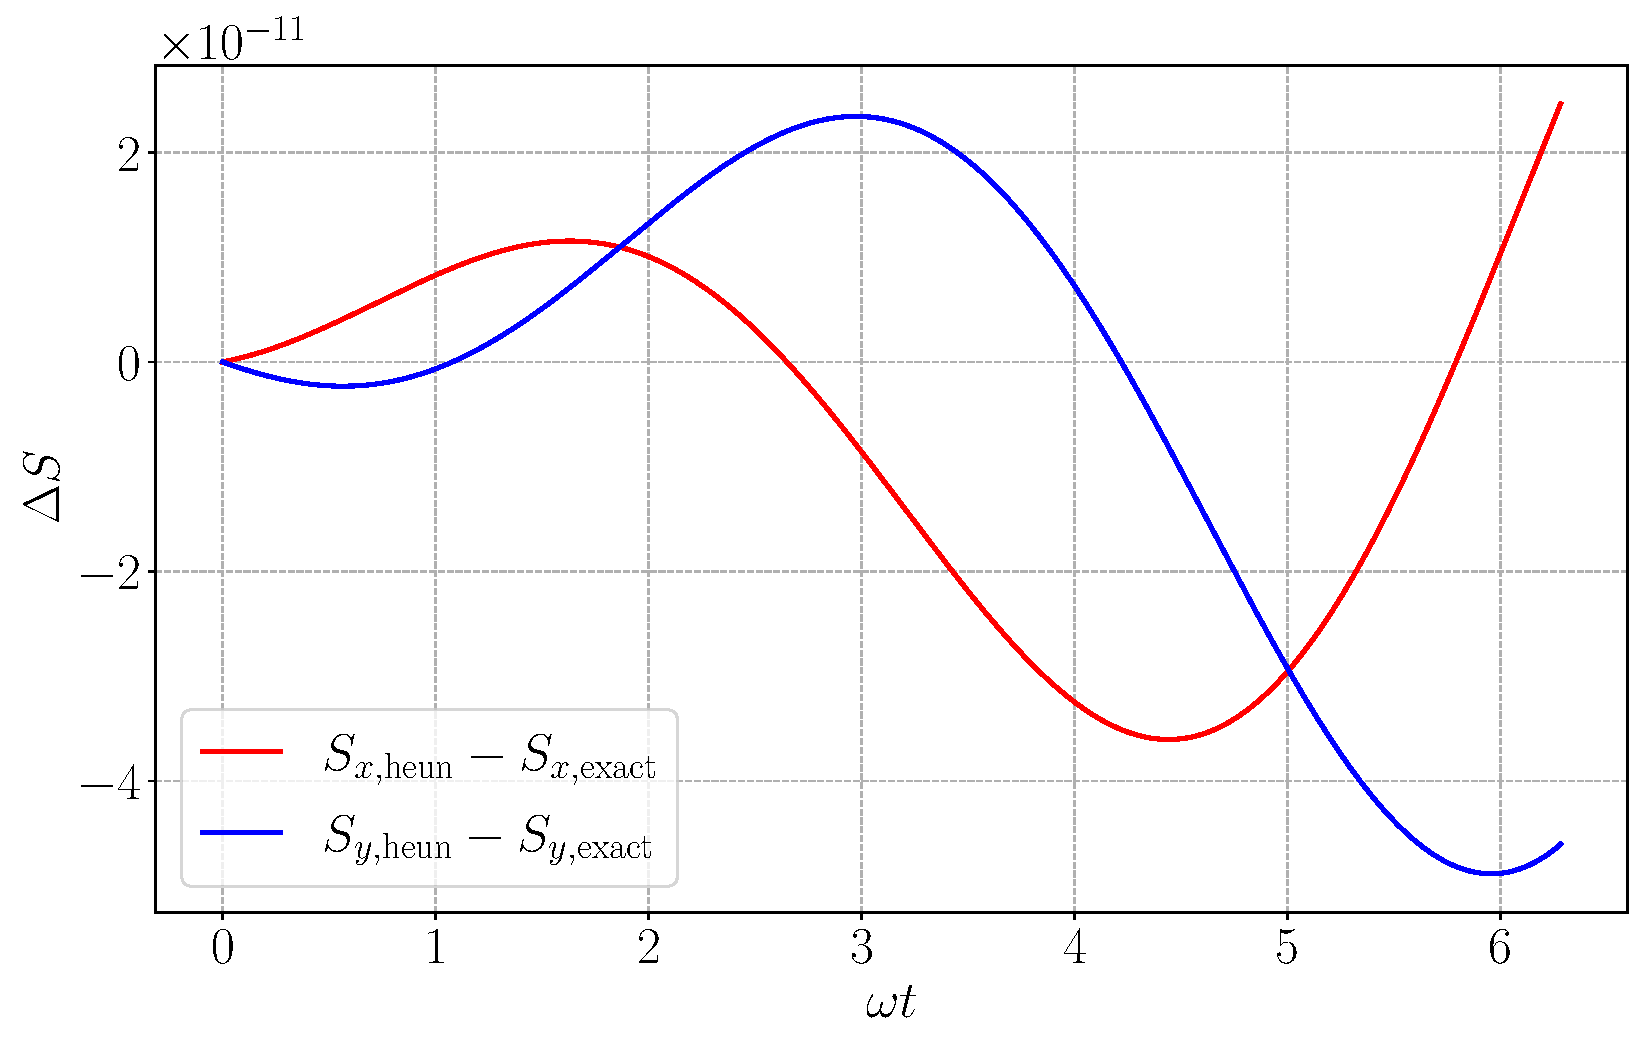
\includegraphics[width=\columnwidth]{../fig/comparison_diff.pdf}
	\caption{The plot shows the difference between the exact solutions given in \eqref{eq:exact_1} and \eqref{eq:exact_2}, and the numerical solutions over one period.}
	\label{fig:comp_diff}
\end{figure} 